\section{Rendimiento y eficiencia}

El núcleo del sistema desarrollado es realmente liviano.
Se trata de un pequeño conjunto de clases en \textbf{PHP} sin ningún tipo de dependencias externas, por lo que su
tiempo de ejecución y consumo de recursos pueden considerarse despreciables.

Sin embargo, tal y como se puede ver en la figura~\ref{fig:chapter_5.2.performance}, la ejecución del sistema está
ligada a las herramientas en la capa de infraestructura, que son las responsables finales de realizar el trabajo.

En este caso, el rendimiento y el consumo de recursos están directamente ligados a las herramientas seleccionadas y al
documento que se esté analizando.

\begin{figure}[ht]
    \begin{center}
        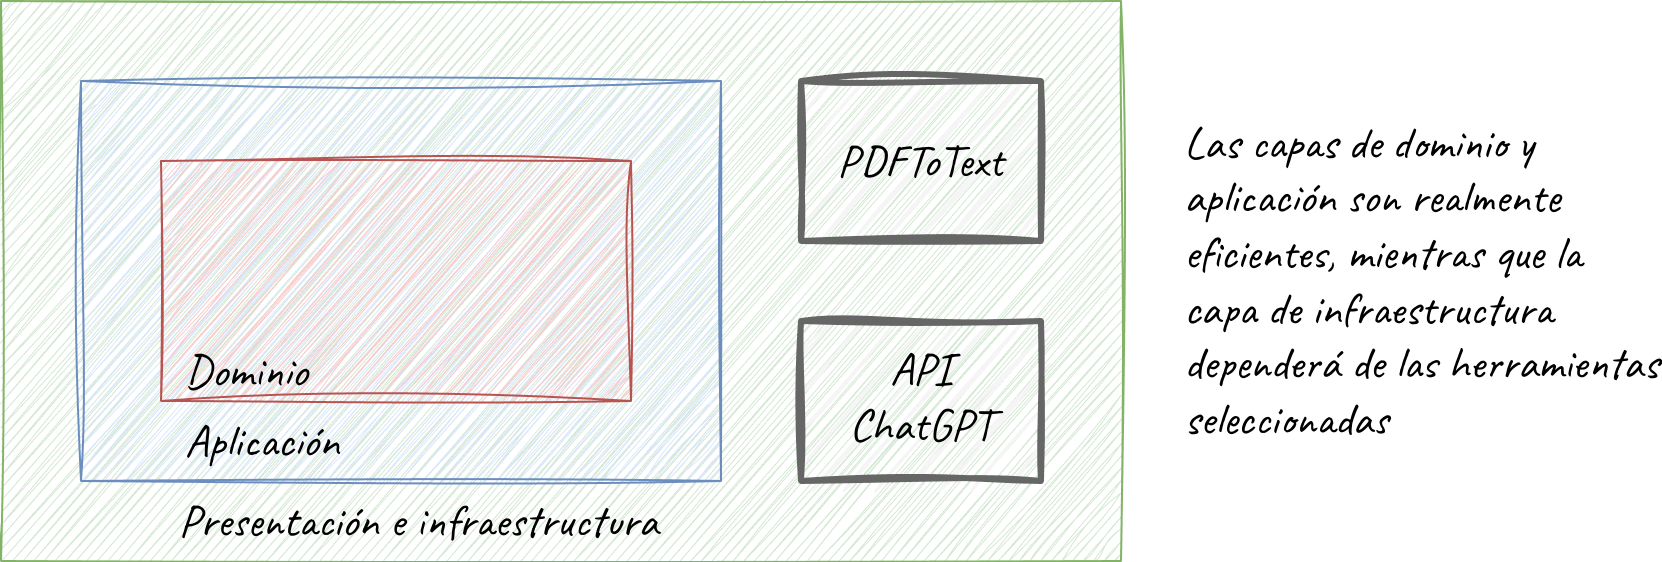
\includegraphics[width=\textwidth]{./chapter/5/images/chapter_5.2.performance}
        \caption{Herramientas en la capa de infraestructura}
        \label{fig:chapter_5.2.performance}
    \end{center}
\end{figure}

El rendimiento también estára relacionado con las características del entorno en el que se está ejecutando y la
carga del mismo.

Sin embargo, hemos calculado los tiempos de ejecución y el consumo de memoria para el documento \textit{001/001.pdf}
con el objetivo de establecer una referencia, tal y como se aprecia en la tabla~\ref{tab:execution_performance}.

\begin{table}[h]
    \renewcommand{\arraystretch}{1.5}
    \setlength{\tabcolsep}{10pt}
    \begin{tabular}{>{\bfseries}p{0.25\textwidth} p{0.20\textwidth} p{0.15\textwidth} p{0.25\textwidth}}
        \toprule
        \textbf{Nombre}                  & \textbf{Ejecución} & \textbf{Memoria} & \textbf{Tiempo}    \\
        \midrule
        \textit{PDF To Text}             & Local              & 288Kb            & 42.49 milisegundos \\
        \textit{API} de \textit{ChatGPT} & Remota             & 612Kb            & 6.74 segundos      \\
        \bottomrule
    \end{tabular}
    \caption{Evaluación del rendimiento de las herramientas en la capa de infraestructura}
    \label{tab:execution_performance}
\end{table}

Como puede verse, el consumo de memoria es realmente bajo, además esta se libera en el momento de completarse cada
ejecución.
Los tiempos de respuesta son muy bajos para \textit{PDF To Text}, que se ejecuta en local, mientras que son bastante
más elevados para los que dependen del consumo de la \textit{API} remota de \textit{ChatGPT}.

Aun así, los tiempos de respuesta para la extracción de la información son realmente buenos si los comparamos con el
tiempo que sería necesario para la extracción por parte de un usuario.

Posiblemente, estos tiempos de respuesta requieran en la mayoría de los casos una ejecución asíncrona, donde el usuario
sube un paquete de documentación y esta se marca con el estado \textit{``PROCESANDO''} mientras que una tarea es
enviada a una cola, donde tras ser ejecutada marcará el paquete como \textit{``PROCESADO''}.
